\documentclass[journal,12pt,twocolumn]{IEEEtran}
%

\usepackage{setspace}
\usepackage{gensymb}
\singlespacing

\usepackage{amsmath}
\usepackage{amsthm}
\usepackage{txfonts}
\usepackage{cite}
\usepackage{enumitem}
\usepackage{mathtools}
\usepackage{listings}
    \usepackage{color}                                            %%
    \usepackage{array}                                            %%
    \usepackage{longtable}                                        %%
    \usepackage{calc}                                             %%
    \usepackage{multirow}                                         %%
    \usepackage{hhline}                                           %%
    \usepackage{ifthen}                                           %%
  %optionally (for landscape tables embedded in another document): %%
    \usepackage{lscape}     
\usepackage{multicol}
\usepackage{chngcntr}
\renewcommand\thesection{\arabic{section}}
\renewcommand\thesubsection{\thesection.\arabic{subsection}}
\renewcommand\thesubsubsection{\thesubsection.\arabic{subsubsection}}

% correct bad hyphenation here
\hyphenation{op-tical net-works semi-conduc-tor}
\def\inputGnumericTable{}                                 %%

\lstset{
%language=C,
frame=single, 
breaklines=true,
columns=fullflexible
}

\begin{document}
%


\newtheorem{theorem}{Theorem}[section]
\newtheorem{problem}{Problem}
\newtheorem{proposition}{Proposition}[section]
\newtheorem{lemma}{Lemma}[section]
\newtheorem{corollary}[theorem]{Corollary}
\newtheorem{example}{Example}[section]
\newtheorem{definition}[problem]{Definition}
\newcommand{\BEQA}{\begin{eqnarray}}
\newcommand{\EEQA}{\end{eqnarray}}
\newcommand{\define}{\stackrel{\triangle}{=}}

\bibliographystyle{IEEEtran}


\providecommand{\mbf}{\mathbf}
\providecommand{\pr}[1]{\ensuremath{\Pr\left(#1\right)}}
\providecommand{\qfunc}[1]{\ensuremath{Q\left(#1\right)}}
\providecommand{\sbrak}[1]{\ensuremath{{}\left[#1\right]}}
\providecommand{\lsbrak}[1]{\ensuremath{{}\left[#1\right.}}
\providecommand{\rsbrak}[1]{\ensuremath{{}\left.#1\right]}}
\providecommand{\brak}[1]{\ensuremath{\left(#1\right)}}
\providecommand{\lbrak}[1]{\ensuremath{\left(#1\right.}}
\providecommand{\rbrak}[1]{\ensuremath{\left.#1\right)}}
\providecommand{\cbrak}[1]{\ensuremath{\left\{#1\right\}}}
\providecommand{\lcbrak}[1]{\ensuremath{\left\{#1\right.}}
\providecommand{\rcbrak}[1]{\ensuremath{\left.#1\right\}}}
\theoremstyle{remark}
\newtheorem{rem}{Remark}
\newcommand{\sgn}{\mathop{\mathrm{sgn}}}
\providecommand{\abs}[1]{\lvert#1\rvert}
\providecommand{\res}[1]{\Res\displaylimits_{#1}} 
\providecommand{\norm}[1]{\lVert#1\rVert}
\providecommand{\mtx}[1]{\mathbf{#1}}
% \providecommand{\mean}[1]{E\left[ #1 \right]}
\providecommand{\fourier}{\overset{\mathcal{F}}{ \rightleftharpoons}}
\providecommand{\system}{\overset{\mathcal{H}}{ \longleftrightarrow}}
\newcommand{\solution}{\noindent \textbf{Solution: }}
\newcommand{\cosec}{\,\text{cosec}\,}
\providecommand{\dec}[2]{\ensuremath{\overset{#1}{\underset{#2}{\gtrless}}}}
\newcommand{\myvec}[1]{\ensuremath{\begin{pmatrix}#1\end{pmatrix}}}
\newcommand{\cmyvec}[1]{\ensuremath{\begin{pmatrix*}[c]#1\end{pmatrix*}}}
\newcommand{\mydet}[1]{\ensuremath{\begin{vmatrix}#1\end{vmatrix}}}
\newcommand{\proj}[2]{\textbf{proj}_{\vec{#1}}\vec{#2}}
\newcommand{\RNum}[1]{\uppercase\expandafter{\romannumeral #1\relax}}
\let\StandardTheFigure\thefigure
\let\vec\mathbf


\title{
\LARGE SM5083\\
    \LARGE Assignment Number 01 \\[0.5em]
    
    \large Deevanshu M.Gupta\par
    \large   SM21MTECH12014  \par
}
\maketitle


\renewcommand{\thefigure}{\theenumi}
\renewcommand{\thetable}{\theenumi}




\section{ chapter \RNum{2}  Q.17 }
\renewcommand{\theequation}{\theenumi}
\begin{enumerate}[label=\thesection.\arabic*.,ref=\thesection.\theenumi]
\numberwithin{equation}{enumi}


\item Show that (2, 4), (3, 0), (5, 3) and (4, 7) are the vertices of a Parallelogram.

\solution
\newline In Fig. 	\ref{fig:3.5.4_quadrilateral1}

let \begin{align}
    \vec{A} = \myvec{2\\4}, \vec{B} = \myvec{3\\0}, \vec{C} = \myvec{5\\3}, \vec{D} = \myvec{4\\7}
\end{align}
$ABCD$ can be a $\parallel$gm if its opposite sides are parallel i.e
\begin{align}
    \vec{A} - \vec{B} = k_1 ( \vec{D} - \vec{C} )\ ~ and ~
    \vec{A} - \vec{D} = k_2 ( \vec{B} - \vec{C} ) 
\end{align}

\begin{align}
\label{eq:constr_vectors_quad1_ABCD}
\vec{A} - \vec{B} = \myvec{-1\\4},~~
\vec{D} - \vec{C} = \myvec{-1\\4}
\\
\vec {A} - \vec {D} = \myvec{-2\\-3},~~
\vec {B} - \vec {C} =\myvec{-2\\-3}
\label{eq:constr_vectors_quad1_ABCD}
\end{align}
From Equation number 1.1.3 and 1.1.4,
\begin{align}
    \vec{A} - \vec{B} &= (1) ( \vec{D} - \vec{C} ) ~and~
    \vec{A} - \vec{D}& = (1) ( \vec{B} - \vec{C} ) 
\end{align}
Here Opposite sides AB $\parallel$ CD and AD $\parallel$ BC 

$\therefore$ $ABCD$ is a $\parallel$gm as the opposite sides are parallel.
%
\item Fig. \ref{fig:3.5.4_quadrilateral1} is generated using 
\begin{lstlisting}
https://github.com/deviith/SM5083/blob/main/Assignment01/Parallelogram.py
\end{lstlisting}
\begin{figure}[!ht]
	\centering
	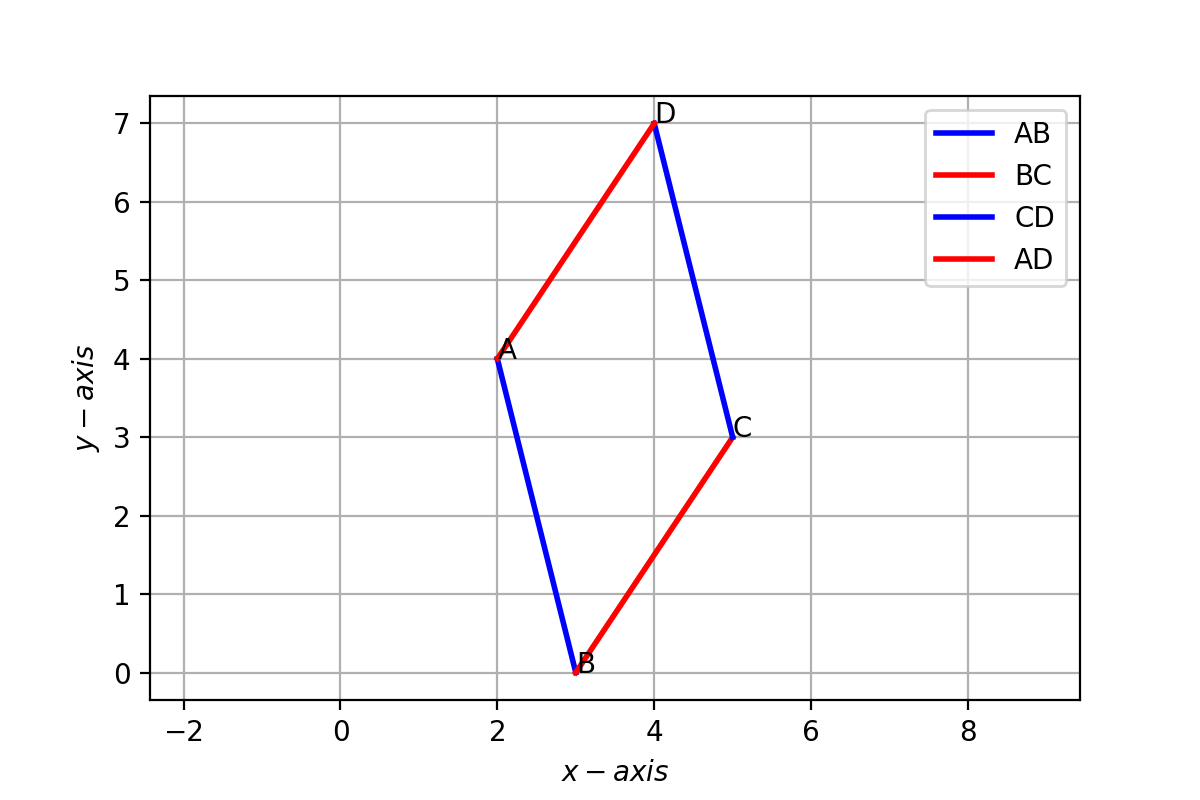
\includegraphics[width=\columnwidth]{Parallelogram.png}
	\caption{The given points form a parallelogram}
	\label{fig:3.5.4_quadrilateral1}
\end{figure}


\end{enumerate}

\end{document}


